\documentclass[11pt,a4paper]{article}

% ── パッケージ ──────────────────────────────────────────
\usepackage[margin=1.1in]{geometry}
\usepackage{amsmath,amssymb,amsthm}
\usepackage{graphicx}
\usepackage{booktabs}
\usepackage{hyperref}
\usepackage[numbers,sort&compress]{natbib}
\usepackage{microtype}
\usepackage{xcolor}
\usepackage[capitalize]{cleveref}
\usepackage{enumitem}
\usepackage{thmtools}
\usepackage{setspace}

% ── ハイパーリンクの色設定 ──────────────────────────────
\hypersetup{
  colorlinks=true,
  linkcolor=blue!60!black,
  citecolor=blue!60!black,
  urlcolor=blue!60!black
}

% ── タイトル ─────────────────────────────────────────────
\title{%
  \textbf{Plausible but Not Brain-Driven:}\\
  \textbf{Quantifying Prior Dominance in Neural Image Reconstruction}
}

\author{
  Yuki Kikuchi\\[0.4em]
  \small\textit{Preprint — 2026}
}

\date{}

% ── 本文 ─────────────────────────────────────────────────
\begin{document}

\maketitle
\thispagestyle{empty}

% ─────────────────────────────────────────────────────────
\begin{abstract}
Brain-to-image reconstruction can produce strikingly realistic images, but it
remains unclear whether these reconstructions are actually driven by brain
signals. Existing metrics primarily assess perceptual similarity (e.g., feature
similarity or visual fidelity), rather than whether brain activity genuinely
controls the output. Strong generative priors can produce plausible images even
when brain activity is randomized---a failure mode that current metrics cannot
detect.

We introduce the \textbf{Degree of Brain Control (BC)}, defined as the ratio of
within-category feature variance under shuffled versus preserved brain--stimulus
correspondence. $\mathrm{BC}=1$ indicates prior-dominated reconstruction,
whereas $\mathrm{BC}>1$ indicates that brain signals impose structure on the
output.

Applied to the GOD dataset, real fMRI yields $\mathrm{BC}=1.259$ while shuffled
signals yield $\mathrm{BC}=1.001$, despite identical feature norms and
comparable visual quality. This dissociation replicates across all five subjects
(paired $t=7.44$, $p=0.0017$). Furthermore, BC captures structural degradation
of decoded representations that is not detectable by identification accuracy
alone ($d=0.465$, $p=0.023$).

BC provides an interpretable absolute scale for quantifying how much brain
signals constrain reconstruction beyond model priors.
\end{abstract}

\newpage
\tableofcontents
\newpage

% ─────────────────────────────────────────────────────────
\section{Introduction}

Brain-to-image reconstruction has progressed from recovering coarse spatial
patterns \citep{miyawaki2008,nishimoto2011} to producing images that appear to
reflect fine-grained visual content
\citep{shen2019,ozcelik2023,scotti2023}. This progress has been driven in large
part by increasingly powerful generative models---GANs, VAEs, and diffusion
models---that serve as the image synthesis stage of reconstruction pipelines.
The reconstructed images are evaluated primarily on visual quality: perceptual
similarity, identification accuracy, or pixel-level fidelity. By these
measures, recent methods appear highly successful.

Yet visual quality is not the same as brain control. A generative model with a
strong prior can produce realistic, category-consistent images even when its
inputs carry no brain-specific information. Consider a decoder that maps fMRI
signals to intermediate features, followed by a generator that reconstructs an
image from those features. If the generator's prior is sufficiently strong, it
will produce a natural-looking image regardless of whether the decoded features
reflect the actual stimulus---simply because the prior constrains the output to
the manifold of natural images. Under these conditions, reconstructions may look
convincing while being dominated by the model prior rather than by brain signals.
Existing metrics---structural similarity (SSIM), perceptual distance (LPIPS,
DreamSim), and identification accuracy---measure properties of the output image,
not the extent to which that output is constrained by brain activity. None can
distinguish a brain-driven reconstruction from a prior-driven one when both
produce visually similar results.

We make this failure mode concrete: when the correspondence between fMRI trials
and stimuli is randomly shuffled, the resulting reconstructions have identical
feature norms and comparable visual quality to those produced by genuine brain
signals---yet by construction contain no stimulus-specific information. Standard
metrics cannot detect this shuffling. This motivates a different question: not
\textit{how realistic} is the reconstruction, but \textit{how much is the
reconstruction controlled by the brain?}

To answer this question, we introduce the \textbf{Degree of Brain Control (BC)},
a metric defined as the ratio of within-category feature variance under shuffled
versus preserved brain--stimulus correspondence. When brain signals carry no
category-relevant information, shuffling does not change the variance structure
of decoded features, and $\mathrm{BC}\approx 1$. When brain signals impose
consistent structure within categories, preserved correspondence yields lower
within-category variance than shuffled correspondence, and $\mathrm{BC}>1$.
$\mathrm{BC}=1$ thus provides an empirically grounded baseline for
prior-dominated reconstruction, and deviations above 1 are directly
interpretable as evidence of brain influence.

We make the following contributions:

\begin{enumerate}[leftmargin=1.5em]
  \item \textbf{Identifying a fundamental failure mode.} We show that
    prior-dominated reconstruction---plausible-looking output with no genuine
    brain influence---is undetectable by existing metrics. This failure mode
    becomes more severe as generative priors grow stronger, making it
    increasingly relevant to the field.

  \item \textbf{BC as the metric that uniquely detects it.} We define BC and
    establish its theoretical grounding, including an information-theoretic
    interpretation ($I(c;\hat{\mathbf{x}})\approx\frac{1}{2}\log\mathrm{BC}$)
    and its relationship to decoder SNR\@. $\mathrm{BC}=1$ provides an
    empirically grounded, interpretable floor for prior-dominated reconstruction.

  \item \textbf{Empirical validation across five subjects.} Real fMRI yields
    $\mathrm{BC}=1.259$; shuffled signals yield $\mathrm{BC}=1.001$---despite
    identical feature norms and comparable visual quality. This dissociation
    replicates across all five subjects (paired $t=7.44$, $p=0.0017$), ruling
    out subject-specific effects.

  \item \textbf{Non-redundancy with identification accuracy.} BC captures
    structural degradation of decoded representations not detectable by
    identification accuracy alone. Matched-accuracy conditions differ
    significantly in BC ($d=0.465$, $p=0.023$), and BC degrades faster than
    accuracy under noise injection---demonstrating that BC and accuracy are
    complementary, not equivalent.
\end{enumerate}

The remainder of this paper is organized as follows. \Cref{sec:related} reviews
related work. \Cref{sec:method} formally defines BC\@. \Cref{sec:experiments}
presents our experiments. \Cref{sec:discussion} discusses implications and
limitations.

% ─────────────────────────────────────────────────────────
\section{Related Work}
\label{sec:related}

\subsection{Brain-to-Image Reconstruction}

Early work on neural image reconstruction focused on recovering low-level visual
features---such as oriented gratings and spatial frequency maps---directly from
fMRI responses using linear models \citep{miyawaki2008,nishimoto2011}. A key
advance came with the introduction of intermediate feature representations:
rather than predicting pixels directly, \citet{shen2019} proposed decoding deep
CNN features (AlexNet layers) from brain signals and inverting them into images
using a feature-to-image generator trained on natural images. This approach,
demonstrated on the Generic Object Decoding (GOD) dataset \citep{shen2019},
produced recognizable object-level reconstructions for the first time at scale.

Subsequent work shifted toward more powerful generative backbones.
Brain-Diffuser \citep{ozcelik2023} and MindEye \citep{scotti2023} leverage
latent diffusion models conditioned on CLIP embeddings decoded from fMRI,
achieving high perceptual quality and identification accuracy. MinD-Vis
\citep{chen2023} similarly exploits masked brain modeling as a pretraining
objective before diffusion-based synthesis. While these methods represent
impressive engineering achievements, they share a common structural property: a
powerful generative prior whose output quality is largely determined by the prior
itself, independent of the quality of the brain-decoded input. Our work
addresses a measurement gap that becomes increasingly important as these priors
grow stronger.

\subsection{Evaluation Metrics for Brain Decoding}

Reconstruction quality in brain decoding is typically assessed along two axes:
pixel-level fidelity and semantic accuracy.

\textbf{Pixel-level metrics} (MSE, SSIM, PSNR) compare reconstructed images to
target images at the pixel level. These metrics are well-understood but poorly
suited to high-level generative pipelines where the output lies on a
low-dimensional natural-image manifold regardless of input quality.

\textbf{Perceptual similarity metrics} (LPIPS \citep{zhang2018}, DreamSim
\citep{fu2023}) measure distance in deep feature spaces and better reflect human
perceptual judgments. However, they still assess how similar the reconstruction
\textit{looks} to the target, not whether the brain signal determined that
appearance.

\textbf{Identification accuracy} (top-$k$ or leave-one-out ranking in feature
space) tests whether the reconstruction is closer to its target image than to
distractors. This has become a standard benchmark \citep{shen2019,scotti2023}.
Yet identification accuracy can be high even when the generator prior contributes
most of the signal: a decoder that consistently maps brain responses to
near-the-mean of the training distribution may still rank correctly if the
distractor features are sufficiently different.

None of these metrics addresses a more fundamental question: \textit{to what
degree are brain signals controlling the reconstruction, rather than the model
prior?} BC is designed to answer exactly this question.

\subsection{Role of Generative Priors}

The tension between model priors and input fidelity is well-recognized in the
generative modeling literature. In VAEs \citep{kingma2014}, the KL
regularization term explicitly pulls latent codes toward a standard Gaussian
prior, reducing the influence of individual inputs. In GANs \citep{goodfellow2014}
and diffusion models \citep{ho2020,song2021}, the prior is implicit but strong:
sampling procedures are designed to produce outputs on the natural-image
manifold. As model capacity increases, these priors become more constraining
relative to the decoder input.

In the brain decoding context, this tension manifests as a trade-off between
visual quality and brain control: stronger priors yield more realistic
reconstructions but may reduce the degree to which individual brain states are
reflected in the output. Several authors have noted informally that
diffusion-based reconstructions may be ``over-smoothed'' toward category
prototypes \citep{ozcelik2023}, but no quantitative metric has been proposed to
measure this effect. BC formalizes this intuition as a measurable, interpretable
quantity.

Concurrent work on hallucination detection in neural decoding \citep{tang2023}
shares the motivation of identifying when generative models produce outputs not
supported by the input signal, but focuses on linguistic decoding rather than
image reconstruction and does not provide a variance-ratio formulation comparable
to BC\@.

% ─────────────────────────────────────────────────────────
\section{Method: Degree of Brain Control}
\label{sec:method}

\subsection{Problem Setup}

Let $\mathbf{b}_i\in\mathbb{R}^V$ denote the fMRI response on trial $i$, and
let $c_i\in\{1,\ldots,C\}$ denote the category label of the presented stimulus.
A reconstruction pipeline consists of two stages: a decoder
$f:\mathbb{R}^V\to\mathbb{R}^d$ that maps brain signals to an intermediate
feature vector, and a generator $g:\mathbb{R}^d\to\mathcal{I}$ that maps
features to image space. In practice, $f$ is a linear (Ridge regression) decoder
trained on held-out data, and the decoded feature
$\hat{\mathbf{x}}_i=f(\mathbf{b}_i)\in\mathbb{R}^d$ is used as input to $g$.

We evaluate brain control at the feature level, i.e., on the set of decoded
features $\{\hat{\mathbf{x}}_i\}$ over $N$ test trials. Let
$S_c=\{i:c_i=c\}$ be the index set of trials belonging to category $c$, with
$|S_c|=n$ for all $c$.

\subsection{Definition}

We define two variance quantities over the decoded features.

\textbf{Within-category variance under preserved correspondence}
($V_\mathrm{pres}$) measures trial-to-trial variability within the same category
when brain signals are correctly paired with stimuli:
\begin{equation}
  V_\mathrm{pres}
  = \frac{1}{C}\sum_{c=1}^{C}\frac{1}{d}\sum_{k=1}^{d}
    \mathrm{Var}_{i\in S_c}[\hat{x}_{ik}].
\end{equation}

\textbf{Within-category variance under broken correspondence}
($V_\mathrm{brok}$) measures the same quantity after randomly permuting the
trial indices, destroying the brain--stimulus pairing:
\begin{equation}
  V_\mathrm{brok}
  = \mathbb{E}_{\pi}\!\left[
    \frac{1}{C}\sum_{c=1}^{C}\frac{1}{d}\sum_{k=1}^{d}
    \mathrm{Var}_{i\in S_c}[\hat{x}_{\pi(i),k}]
  \right],
\end{equation}
where $\pi$ is a uniformly random permutation of $\{1,\ldots,N\}$. The
expectation is estimated by averaging over $N_\mathrm{shuf}=1000$ independent
permutations.

The \textbf{Degree of Brain Control} is defined as:
\begin{equation}
  \boxed{
    \mathrm{BC} = \frac{V_\mathrm{brok}}{V_\mathrm{pres}}
  }
  \label{eq:bc}
\end{equation}

\subsection{Interpretation}

\textbf{$\mathrm{BC}=1$} (prior-dominated): Shuffling trial indices does not
change the variance structure of decoded features. The decoder output carries no
category-specific information---reconstruction is determined entirely by the
model prior, not by the brain signals.

\textbf{$\mathrm{BC}>1$} (brain-controlled): Preserved correspondence yields
lower within-category variance than broken correspondence. Trials within the same
category produce more similar decoded features when correctly paired with their
stimuli than when randomly paired. This indicates that brain signals impose
consistent structure on the reconstruction.

The quantity $\mathrm{BC}-1$ serves as an effect-size measure of brain influence.
Under a Gaussian approximation of the feature distribution, BC has a direct
information-theoretic interpretation:
\begin{equation}
  I(c;\,\hat{\mathbf{x}})
  \approx \frac{1}{2}\log\mathrm{BC},
  \label{eq:mi}
\end{equation}
where $I(c;\hat{\mathbf{x}})$ is the mutual information between the category
label and the decoded feature vector. $\mathrm{BC}=1$ corresponds to zero mutual
information; $\mathrm{BC}>1$ corresponds to positive information transmission
from stimulus category through brain signals to decoded features.

\subsection{Relationship to Identification Accuracy}

Identification accuracy (e.g., leave-one-out cosine similarity ranking) is a
commonly used metric in brain decoding. Both BC and accuracy increase with the
signal-to-noise ratio of the decoder. However, identification accuracy is a
nonlinear (sigmoidal) function of SNR and saturates at high SNR, whereas BC
scales approximately linearly:
\begin{equation}
  \mathrm{BC} \approx 1 + \mathrm{SNR}_\mathrm{eff},
\end{equation}
where $\mathrm{SNR}_\mathrm{eff}$ is the effective signal-to-noise ratio in
feature space. This means BC continues to grow in regimes where accuracy has
already saturated, enabling detection of structural differences that accuracy
cannot resolve. We demonstrate this empirically in \cref{sec:exp2}.

\subsection{Computation}

Given $N$ test trials with decoded features $\{\hat{\mathbf{x}}_i\}$ and
category labels $\{c_i\}$:
\begin{enumerate}[leftmargin=1.5em]
  \item Compute $V_\mathrm{pres}$ directly from the decoded features.
  \item Estimate $V_\mathrm{brok}$ by averaging over $N_\mathrm{shuf}=1000$
    random permutations.
  \item Compute $\mathrm{BC}=V_\mathrm{brok}/V_\mathrm{pres}$.
\end{enumerate}
Category-level BC values $\{\mathrm{BC}_c\}$ are computed per category and
averaged; these are also used for effect-size analyses (Cohen's $d$). The
shuffle-based standard error provides an uncertainty estimate for BC\@.

% ─────────────────────────────────────────────────────────
\section{Experiments}
\label{sec:experiments}

\subsection{Setup}

\textbf{Dataset.} We use the Generic Object Decoding (GOD) dataset
\citep{shen2019}, which contains fMRI responses from five subjects viewing 1,200
training images and 50 test images (one image per category, repeated 35 times
each). Test trials thus consist of $50\times35=1{,}750$ trials per subject. All
analyses use the Visual Cortex (VC) ROI unless otherwise stated.

\textbf{Decoder.} We train a Ridge regression decoder ($\alpha=100$) with
standard scaling to predict AlexNet relu7 features (fc7, $d=4{,}096$) from brain
signals. The decoder is trained on training-set trials and evaluated on held-out
test trials, following the original GOD experimental protocol \citep{shen2019}.

\textbf{BC computation.} For each experiment, BC is computed using
$N_\mathrm{shuf}=1{,}000$ across-trial permutations (\cref{eq:bc}). Category-level
BC values are averaged to obtain a scalar summary; their standard error across
categories provides an uncertainty estimate.

\subsection{Experiment 1: Prior-Dominated Baseline}
\label{sec:exp1}

\textbf{Setup.} We compare three conditions that differ only in the brain signals
fed to the decoder:
\begin{itemize}[leftmargin=1.5em]
  \item \textbf{Real}: genuine fMRI test signals (correct brain--stimulus
    pairing).
  \item \textbf{Shuffled}: test trial indices randomly permuted before decoding,
    destroying brain--stimulus correspondence while preserving the marginal
    distribution of brain signals.
  \item \textbf{Random}: standard Gaussian noise substituted for brain signals,
    representing complete absence of brain information.
\end{itemize}
The decoder and generator are identical across all three conditions.

\textbf{Results.}

\begin{table}[h]
\centering
\caption{BC and feature norm across three input conditions (Subject 1, VC ROI).}
\label{tab:main}
\begin{tabular}{lcc}
\toprule
Condition & BC & Feature norm (L2) \\
\midrule
Real      & \textbf{1.259} & 70.9 \\
Shuffled  & 1.001          & 70.9 \\
Random    & 1.000          & 118.4 \\
\bottomrule
\end{tabular}
\end{table}

The key finding is the dissociation between BC and feature norm
(\cref{tab:main}). Real and Shuffled conditions produce decoded features with
identical L2 norms (70.9), meaning that any metric based on feature
magnitude---and by extension, visual quality---cannot distinguish them. Yet BC
separates them sharply: Real yields $\mathrm{BC}=1.259$, while Shuffled yields
$\mathrm{BC}=1.001$, consistent with pure prior domination ($\mathrm{BC}=1$ by
construction when correspondence is destroyed).

\Cref{fig:recon} shows reconstructed images for three representative categories
under all three conditions. Rows are visually similar across conditions,
confirming that feature norm (and visual quality) is insufficient to distinguish
brain-controlled from prior-dominated reconstruction. \Cref{fig:barplot} presents
the BC and feature norm comparison as bar charts, making the dissociation
explicit.

\begin{figure}[t]
\centering
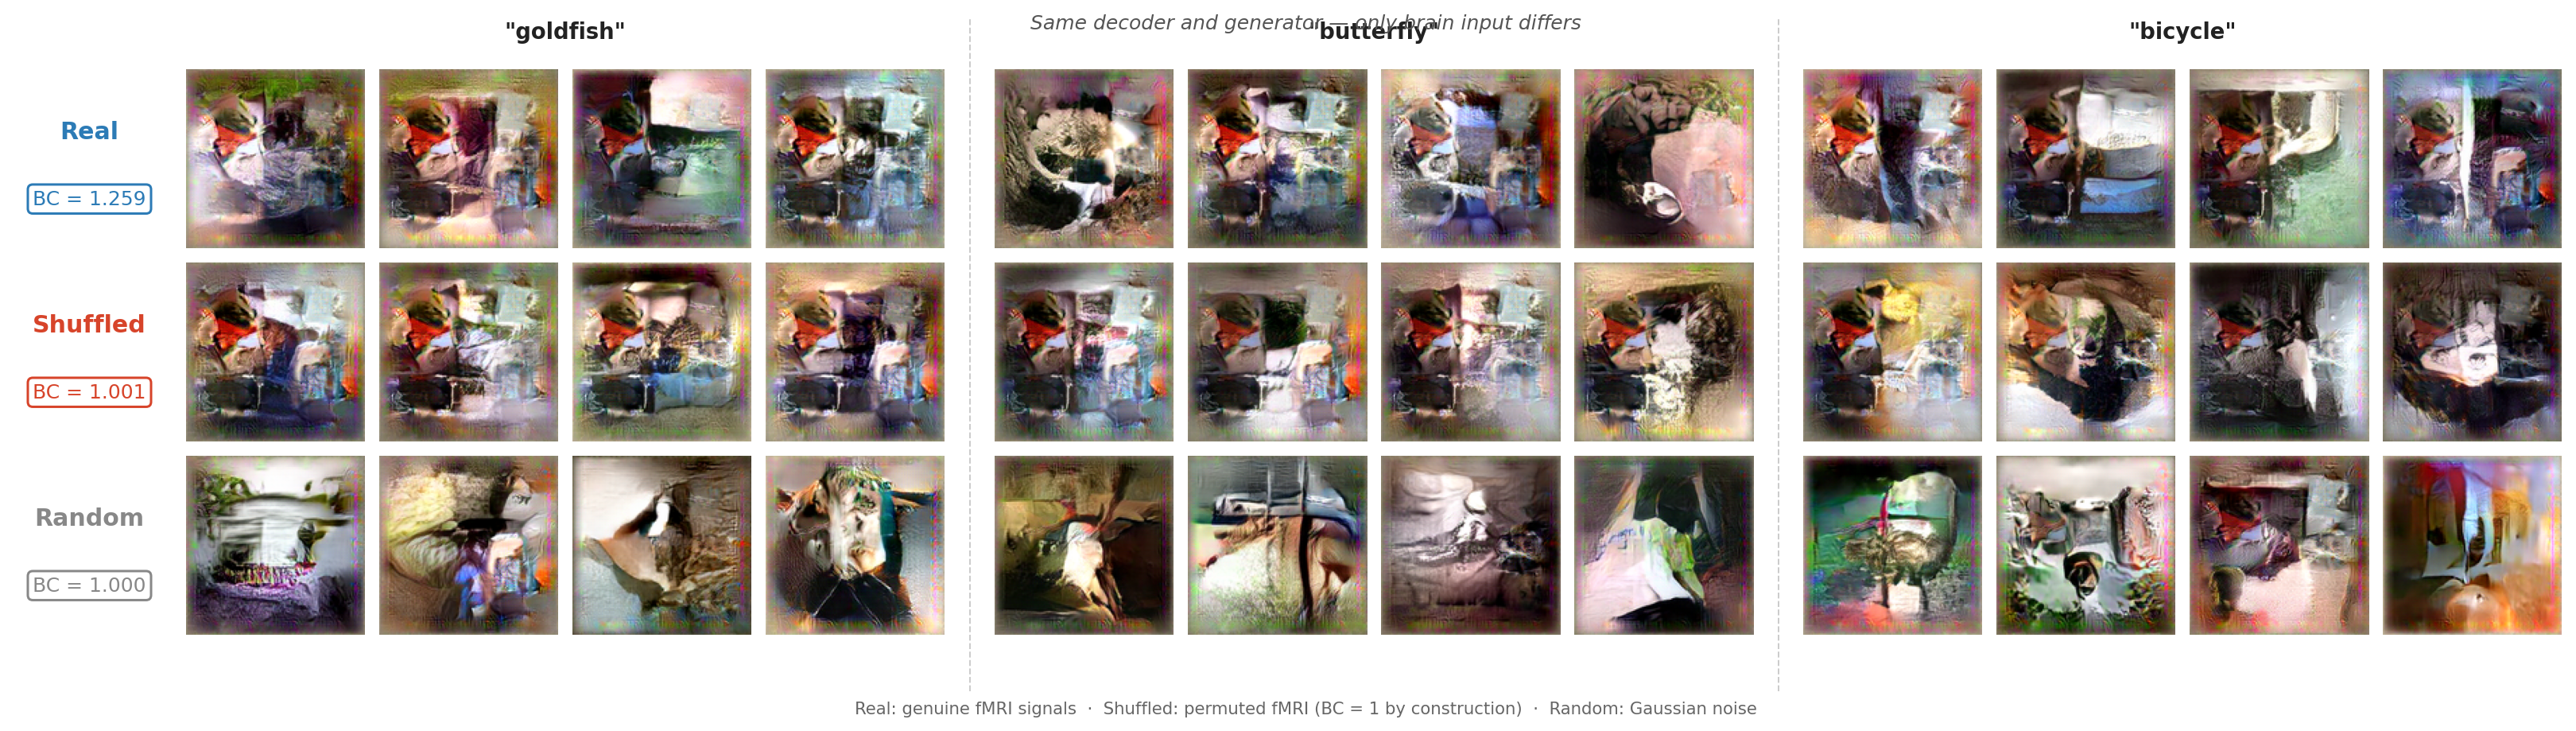
\includegraphics[width=\linewidth]{fig2_reconstruction_comparison.png}
\caption{Reconstructed images under three input conditions (Real, Shuffled,
  Random) for three representative categories (goldfish, butterfly, bicycle),
  showing four repetitions each. Rows are visually similar across conditions
  despite the large difference in BC, demonstrating that visual quality cannot
  distinguish brain-controlled from prior-dominated reconstruction.}
\label{fig:recon}
\end{figure}

\begin{figure}[t]
\centering
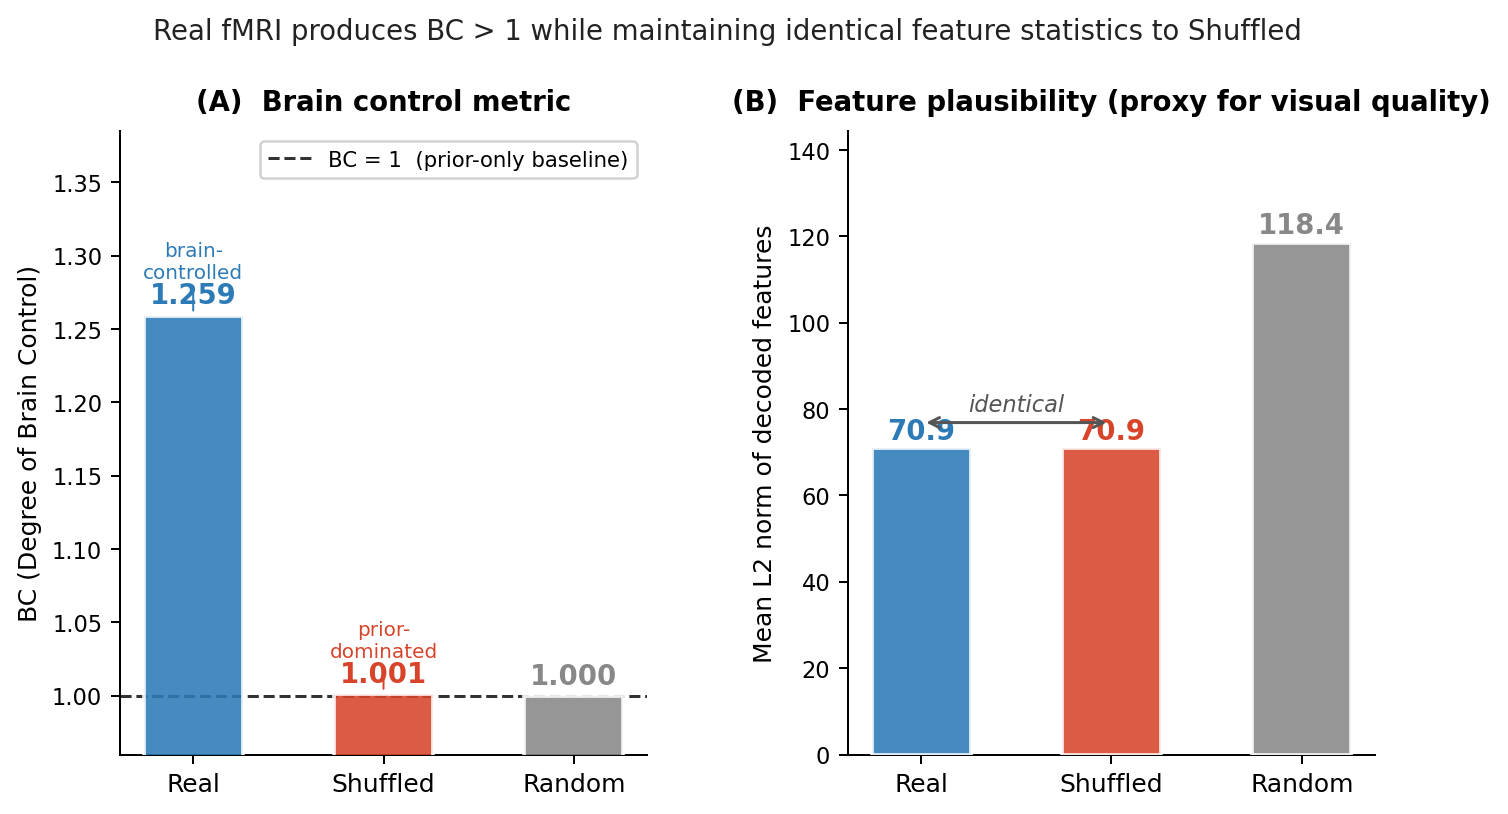
\includegraphics[width=0.85\linewidth]{fig3_bc_barplot.png}
\caption{(A) BC and (B) feature L2 norm across three conditions. Real and
  Shuffled conditions have identical feature norms (right panel), yet BC
  distinguishes them sharply (left panel). The dashed line indicates
  $\mathrm{BC}=1$ (prior-only baseline).}
\label{fig:barplot}
\end{figure}

\textbf{Multi-subject replication.} To assess generalizability, we repeat
Experiment~1 for all five subjects in the GOD dataset (\cref{tab:multisubj}).
Real BC exceeds Shuffled BC in every subject without exception. A paired
$t$-test across subjects yields $t=7.44$, $p=0.0017$, confirming that the
Real--Shuffled dissociation is not specific to a single subject.

\begin{table}[h]
\centering
\caption{BC across five subjects (VC ROI). Shuffled BC $\approx 1.000$ in all
  subjects; feature norms of Real and Shuffled are identical within each subject.}
\label{tab:multisubj}
\begin{tabular}{lccc}
\toprule
Subject & Real BC & Shuffled BC & Feature norm (Real = Shuffled) \\
\midrule
Subject 1 & 1.259 & 1.001 & 70.9 \\
Subject 2 & 1.135 & 0.999 & 86.4 \\
Subject 3 & 1.250 & 0.999 & 83.5 \\
Subject 4 & 1.208 & 1.001 & 92.9 \\
Subject 5 & 1.138 & 1.002 & 84.0 \\
\midrule
\multicolumn{4}{l}{\small Paired $t$-test (Real vs.\ Shuffled): $t=7.44$, $p=0.0017$} \\
\bottomrule
\end{tabular}
\end{table}

\subsection{Experiment 2: BC vs.\ Identification Accuracy}
\label{sec:exp2}

\textbf{Motivation.} A natural concern is that BC may be redundant with
identification accuracy. We investigate the relationship between the two metrics
and examine whether BC provides information beyond what accuracy already captures.

\textbf{ROI comparison.} We compute both BC and leave-one-out cosine similarity
accuracy across ten visual ROIs (V1, V2, V3, V4, LOC, FFA, PPA, LVC, HVC, VC)
for Subject~1. Across ROIs, BC and accuracy are highly correlated ($r=0.967$),
which is expected: both reflect the quality of the decoded representation and
both are computed from the same Ridge decoder. This high correlation provides a
basic validity check---BC is not measuring noise.

However, correlation does not imply equivalence. BC and accuracy measure
different properties: accuracy captures the ability to rank the correct image
above distractors, while BC measures the absolute variance compression imposed
by brain signals within categories.

\textbf{Same accuracy, different BC.} To demonstrate the non-redundancy of BC
directly, we inject Gaussian noise ($\sigma=0.75$) into standardized V1 signals
and identify the noise level at which V1+noise matches the identification
accuracy of the HVC ROI. Despite being matched in accuracy, V1+noise and HVC
differ significantly in BC (Cohen's $d=0.465$, 95\%~CI~$=[0.003, 0.043]$,
$p=0.023$, two-sample $t$-test over per-category BC values). Two conditions can
have equivalent identification accuracy while differing in the structural quality
of their decoded representations---a difference that BC captures and accuracy
cannot.

\Cref{fig:noise} shows the full noise sensitivity curves. BC degrades faster and
more continuously than accuracy under noise injection, confirming the theoretical
prediction that BC tracks SNR linearly while accuracy tracks it sigmoidally.
\Cref{fig:scatter} shows the BC--accuracy scatter across ROIs, with the
matched-accuracy comparison highlighted.

\begin{figure}[t]
\centering
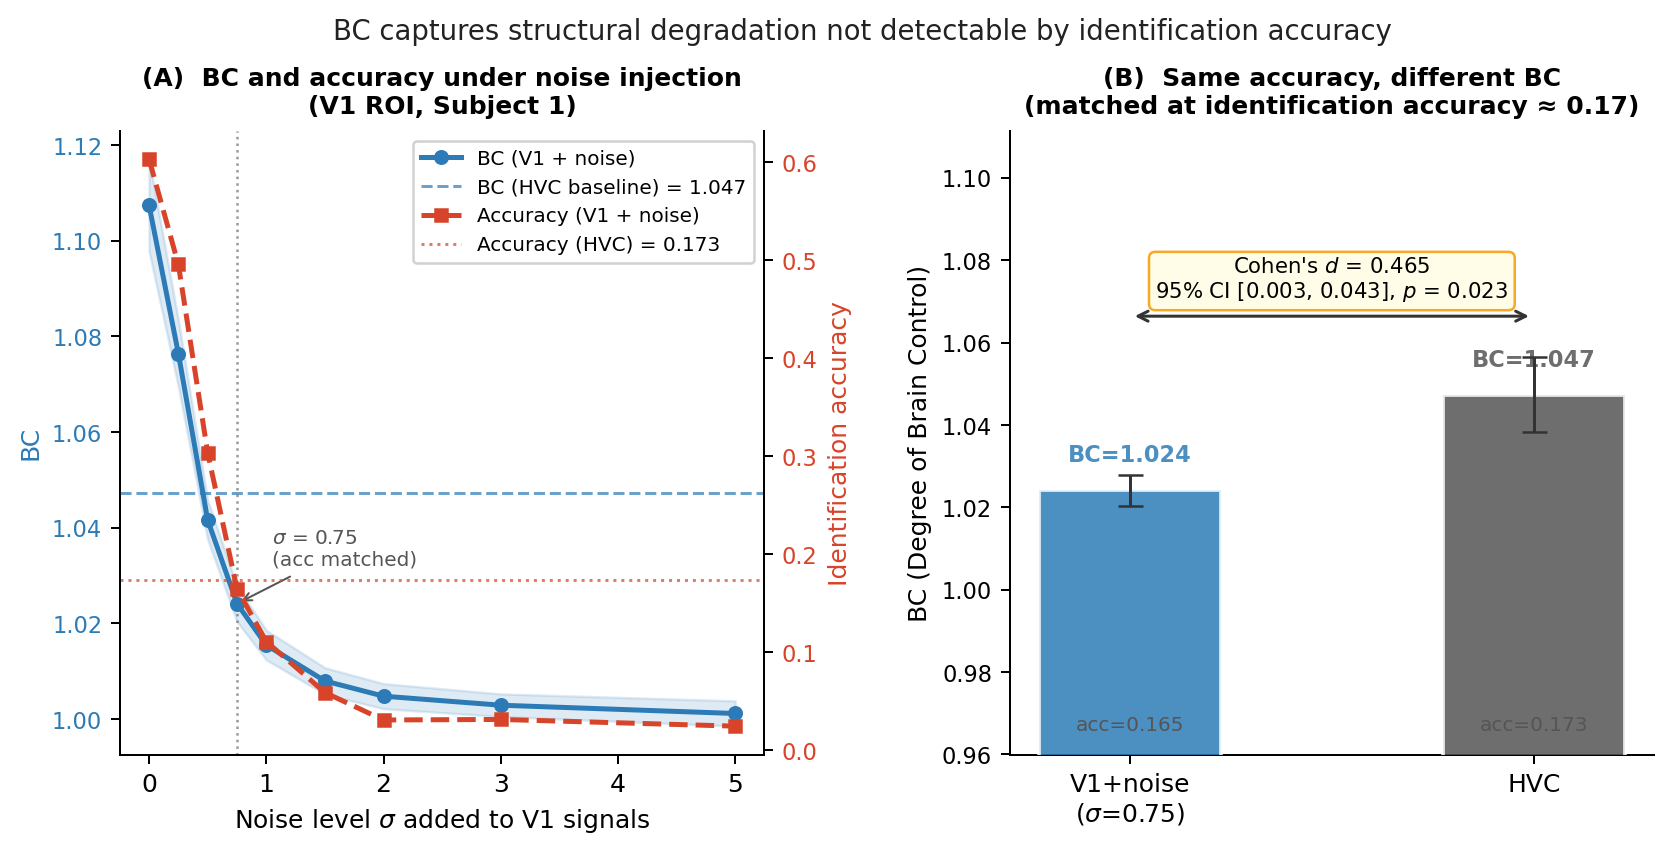
\includegraphics[width=\linewidth]{fig4_noise_sensitivity.png}
\caption{(A) BC (blue) and identification accuracy (red) as a function of noise
  level $\sigma$ added to V1 signals, together with HVC baselines (dashed).
  BC degrades faster than accuracy. (B) At $\sigma=0.75$, accuracy is matched
  between V1+noise and HVC, but BC differs significantly
  ($d=0.465$, $p=0.023$).}
\label{fig:noise}
\end{figure}

\begin{figure}[t]
\centering
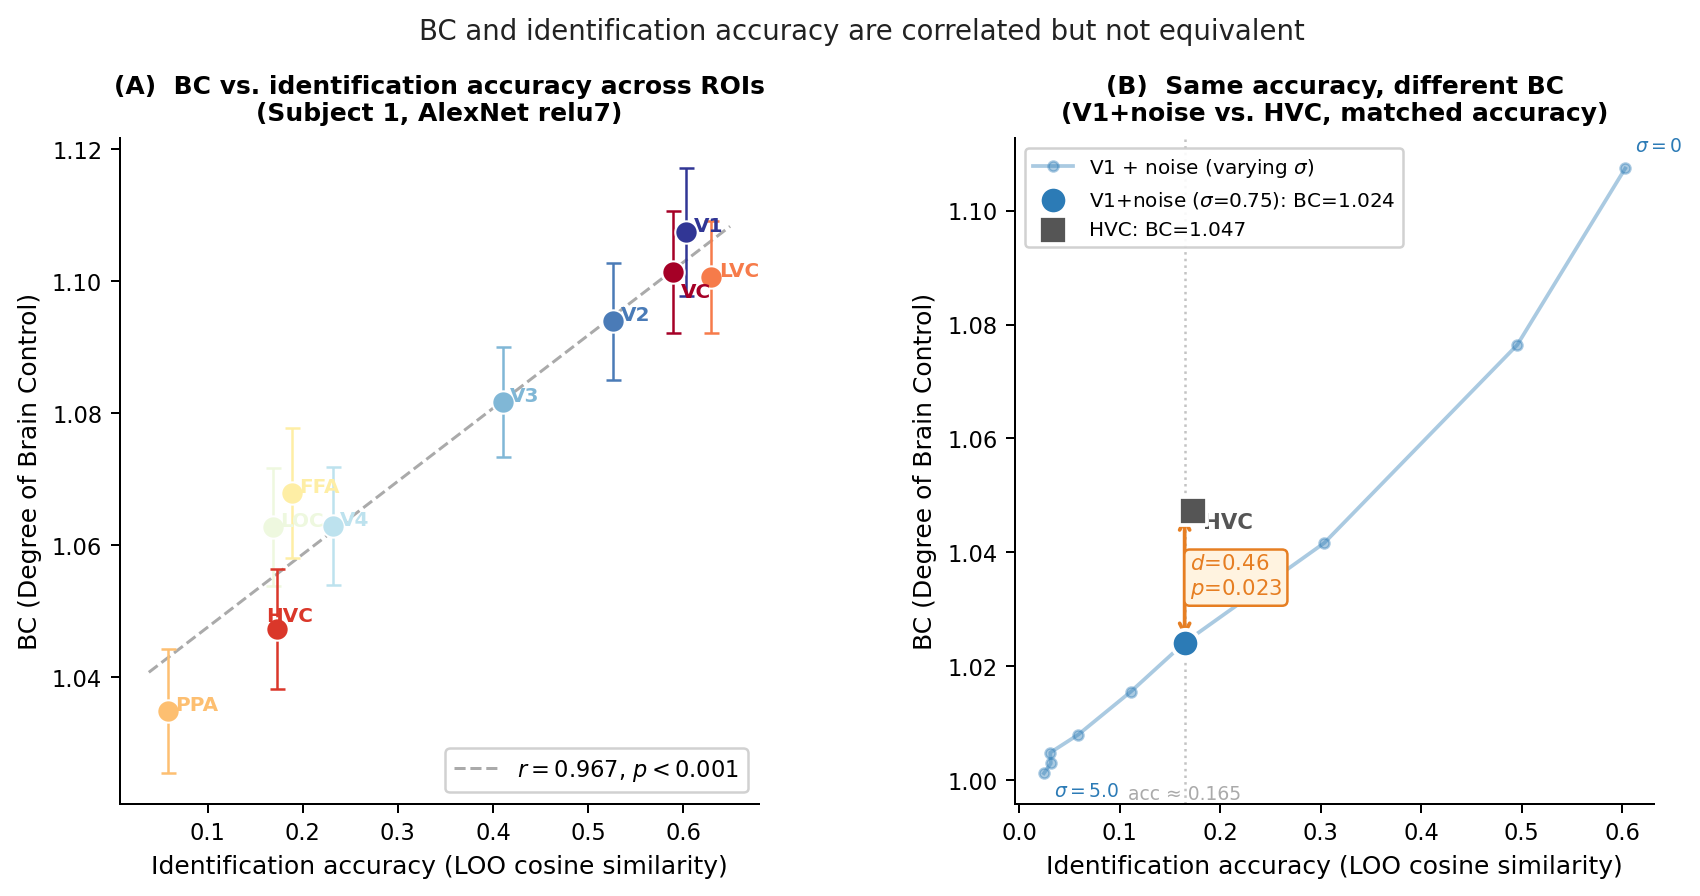
\includegraphics[width=\linewidth]{fig5_bc_vs_accuracy.png}
\caption{(A) BC vs.\ identification accuracy across ten visual ROIs ($r=0.967$).
  (B) The matched-accuracy comparison: V1+noise and HVC have the same accuracy
  but different BC, demonstrating non-redundancy.}
\label{fig:scatter}
\end{figure}

\subsection{Experiment 3: Image-Space Brain Control (Phase 2 BC)}

\textbf{Setup.} Experiments 1--2 measure BC in the intermediate feature space
(relu7, Phase~1 BC). To assess whether brain control extends to the final image
space, we define Phase~2 BC using DreamSim embeddings \citep{fu2023}
($d=1{,}792$) computed directly from generated images.

\textbf{Results.} Phase~2 BC across 50 categories has mean
$1.037\pm0.107$ (std). The per-category distribution is wide: goldfish reaches
$\mathrm{BC}=1.295$ while washer reaches $\mathrm{BC}=0.850$ (below~1,
indicating that the generator introduces category-inconsistent variation not
present in feature space). The correlation between Phase~1 and Phase~2 BC across
categories is $r=0.308$ ($p=0.030$), indicating a weak but significant positive
relationship.

The modest Phase~1--Phase~2 correlation suggests that feature-space brain
control does not fully transfer to image-space brain control. This motivates
measuring BC at both stages of the pipeline when evaluating reconstruction
methods.

% ─────────────────────────────────────────────────────────
\section{Discussion}
\label{sec:discussion}

\subsection{What BC Measures---and What It Does Not}

BC is a variance ratio, not a proportion of variance explained. A value of
$\mathrm{BC}=1.259$ does not mean ``25.9\% of the reconstruction is
brain-controlled.'' It means that within-category feature variance is 25.9\%
higher when brain--stimulus correspondence is destroyed than when it is
preserved---that is, genuine brain signals make same-category reconstructions
more similar to each other than random pairing would. $\mathrm{BC}-1$ is best
interpreted as an effect-size measure of brain influence in feature space,
directly analogous to a signal-to-noise ratio in the decoded representation.

Crucially, $\mathrm{BC}=1$ is not simply a null result; it is an empirically
grounded floor. When brain signals carry no category-relevant information---as in
the Shuffled condition---$\mathrm{BC}=1$ by construction, regardless of how
realistic the reconstructions appear. Any reconstruction pipeline that yields
$\mathrm{BC}\approx 1$ on genuine brain data should be considered
prior-dominated, regardless of its visual quality or identification accuracy.

\subsection{Implications for Diffusion-Based Reconstruction}

The most visually impressive brain reconstruction methods today rely on latent
diffusion models \citep{ozcelik2023,scotti2023}. These models have extremely
strong priors---trained on billions of images and optimized to produce outputs
precisely on the natural-image manifold. This is precisely the regime where BC
is most informative: as the prior strengthens, the generator becomes increasingly
capable of producing high-quality, category-consistent images from near-arbitrary
inputs, and BC should approach~1 even for genuine brain signals.

To empirically ground this prediction, we simulate increasing prior dominance via
feature mixing. We linearly interpolate decoded features between the Real
condition ($\alpha=0$) and the Shuffled condition ($\alpha=1$, prior-dominated
by construction):
\begin{equation}
  \hat{\mathbf{x}}_\alpha
  = (1-\alpha)\,\hat{\mathbf{x}}_\mathrm{real}
  + \alpha\,\hat{\mathbf{x}}_\mathrm{shuffled}.
\end{equation}
As $\alpha$ increases from 0 to 1, BC decreases monotonically from 1.259 to
1.001 (\cref{fig:prior_strength}A), with a near-linear trajectory
(\cref{fig:prior_strength}B). This demonstrates that BC is a continuous,
sensitive measure of prior dominance: any generative process that partially
replaces brain-specific information with prior-driven information will produce a
BC value proportional to the degree of replacement.

This directly supports the prediction that diffusion-based reconstruction
methods---whose stronger generative priors impose more structure on the output
independently of the input---will yield BC values closer to 1 than the
relu7generator used here, despite achieving higher perceptual quality and
identification accuracy. Applying BC to publicly available diffusion-based
reconstructions remains an important direction for future work.

\begin{figure}[t]
\centering
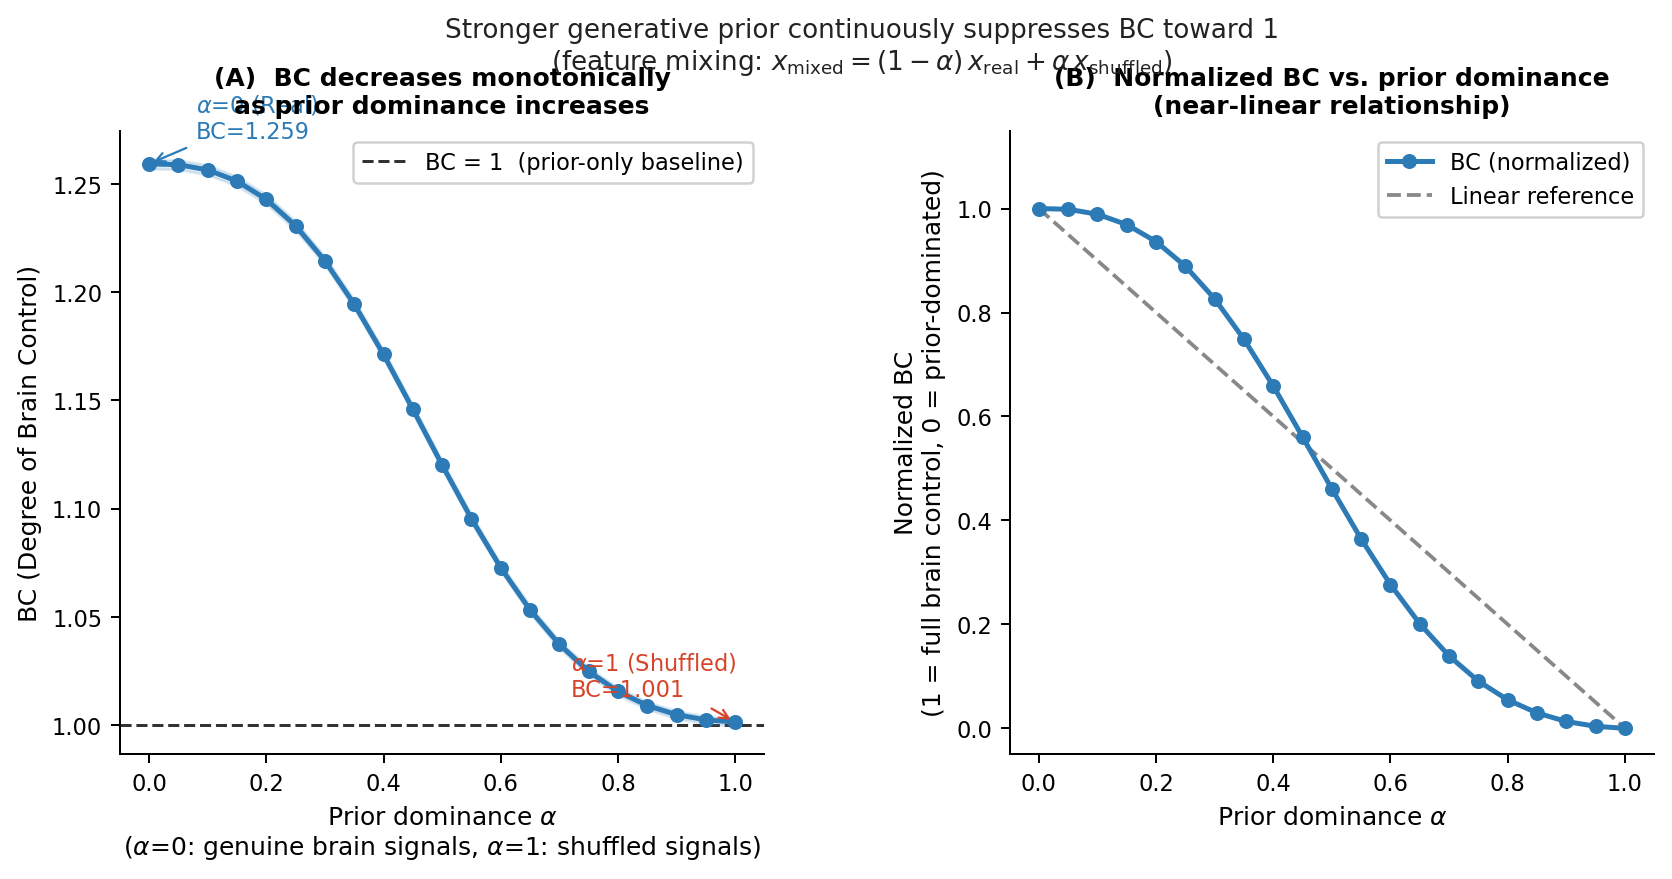
\includegraphics[width=\linewidth]{fig6_prior_strength.png}
\caption{(A) BC as a function of prior dominance $\alpha$, where
  $\hat{\mathbf{x}}_\alpha = (1-\alpha)\hat{\mathbf{x}}_\mathrm{real} +
  \alpha\hat{\mathbf{x}}_\mathrm{shuffled}$. BC decreases monotonically from
  1.259 ($\alpha=0$, full brain control) to 1.001 ($\alpha=1$, prior-dominated).
  (B) Normalized BC shows a near-linear relationship with prior dominance,
  confirming that BC is a continuous, sensitive measure of the brain--prior
  trade-off.}
\label{fig:prior_strength}
\end{figure}

\subsection{BC Beyond the Feature Decoder}

Our results show a weak but significant correlation between Phase~1 BC and
Phase~2 BC ($r=0.308$, $p=0.030$). The modest correlation indicates that brain
control in feature space does not fully transfer to image space---the generator
introduces additional variability that can either amplify or dilute the brain
signal depending on the category. Phase~2 BC, measured directly on generated
images, captures complementary information about the full pipeline and should be
reported alongside Phase~1 BC when the generator is not a simple deterministic
inversion.

\subsection{Limitations}

\textbf{Linear decoder.} BC as computed here depends on the Ridge regression
decoder. A more expressive decoder could extract more category-relevant
information from brain signals, increasing BC\@. Our results represent a lower
bound on the brain control achievable with the GOD dataset and AlexNet features.

\textbf{Feature space selection.} BC is measured in the AlexNet relu7 space.
Different feature spaces may yield different BC values; in particular,
higher-level semantic features (e.g., CLIP embeddings) may show higher BC
because they are more directly predictable from high-level visual cortex
activity. The choice of feature space should be reported when comparing BC values
across studies.

\textbf{Absolute scale.} While BC provides an absolute scale relative to the
prior-dominated baseline ($\mathrm{BC}=1$), the numerical value of
$\mathrm{BC}-1$ is not directly comparable across datasets, decoders, or feature
spaces. BC is most informative as a within-study comparison.

% ─────────────────────────────────────────────────────────
\section{Conclusion}

Brain-to-image reconstruction has made remarkable progress, but visual quality
alone cannot tell us whether the brain is actually driving the output. We
introduced the Degree of Brain Control (BC), a metric that directly addresses
this question by comparing within-category feature variance under preserved
versus shuffled brain--stimulus correspondence. $\mathrm{BC}=1$ provides an
empirically grounded floor corresponding to pure prior-dominated generation;
$\mathrm{BC}>1$ indicates that brain signals impose measurable structure on the
reconstruction.

Applied to the GOD dataset, genuine fMRI signals yield $\mathrm{BC}=1.259$,
while shuffled signals yield $\mathrm{BC}=1.001$---despite producing decoded
features with identical norms and visually indistinguishable reconstructions.
This dissociation, replicated across all five subjects ($t=7.44$, $p=0.0017$),
shows that BC detects a property of brain decoding that no existing metric
captures. Furthermore, BC reveals structural degradation not detectable by
identification accuracy alone ($d=0.465$, $p=0.023$), demonstrating that the two
metrics are complementary rather than redundant.

As generative priors in brain reconstruction grow stronger, the risk of
conflating visual quality with brain control will only increase. We argue that BC
should be reported alongside perceptual quality metrics in all brain-to-image
reconstruction studies, and that maximizing BC---not just visual
fidelity---should be an explicit goal of future decoder development.

% ─────────────────────────────────────────────────────────
\bibliographystyle{plainnat}
\bibliography{references}

\end{document}
